\documentclass[twoside]{article}

\usepackage{aistats2020}


\usepackage{graphicx}
\usepackage[utf8]{inputenc} % allow utf-8 input
\usepackage[T1]{fontenc}    % use 8-bit T1 fonts
\usepackage{hyperref}       % hyperlinks
\usepackage{url}            % simple URL typesetting
\usepackage{booktabs}       % professional-quality tables
\usepackage{amsmath,amssymb} 
\usepackage{amsthm}    % blackboard math symbols
\usepackage{nicefrac}       % compact symbols for 1/2, etc.
\usepackage{microtype}      % microtypography
\usepackage{bm}
\usepackage{subfig}
\usepackage[english]{babel}
\usepackage{algorithm}
%\usepackage{algorithmic}
\usepackage{appendix}

\theoremstyle{plain}
\newtheorem{thm}{Theorem}[section]
\newtheorem{lem}{Lemma}
\newtheorem{prop}{Proposition}
\newtheorem{pro}{Property}
\newtheorem{assumption}{Assumption}

\theoremstyle{definition}
\newtheorem{defn}{Definition}
\newtheorem{cor}{Corollary}
\newtheorem{example}{Example}
\newtheorem{rmk}{Remark}

\input macros.tex
\usepackage{dsfont}

\usepackage{multirow}
\usepackage{algpseudocode,algorithm}
\algnewcommand\algorithmicinput{\textbf{Input:}}
\algnewcommand\algorithmicoutput{\textbf{Output:}}
\algnewcommand\INPUT{\item[\algorithmicinput]}
\algnewcommand\OUTPUT{\item[\algorithmicoutput]}

\DeclareMathOperator*{\minimize}{minimize}



\usepackage{mathtools}
\mathtoolsset{showonlyrefs}
\newcommand*{\KeepStyleUnderBrace}[1]{%f
  \mathop{%
    \mathchoice
    {\underbrace{\displaystyle#1}}%
    {\underbrace{\textstyle#1}}%
    {\underbrace{\scriptstyle#1}}%
    {\underbrace{\scriptscriptstyle#1}}%
  }\limits
}
\usepackage{xr}
\externaldocument{tensor_regression_supp}

% If your paper is accepted, change the options for the package
% aistats2020 as follows:
%
% \usepackage[accepted]{aistats2020}
%
% This option will print headings for the title of your paper and
% headings for the authors names, plus a copyright note at the end of
% the first column of the first page.

% If you set papersize explicitly, activate the following three lines:
%\special{papersize = 8.5in, 11in}
%\setlength{\pdfpageheight}{11in}
%\setlength{\pdfpagewidth}{8.5in}

% If you use natbib package, activate the following three lines:
%\usepackage[round]{natbib}
%\renewcommand{\bibname}{References}
%\renewcommand{\bibsection}{\subsubsection*{\bibname}}

% If you use BibTeX in apalike style, activate the following line:
%\bibliographystyle{apalike}

\begin{document}

% If your paper is accepted and the title of your paper is very long,
% the style will print as headings an error message. Use the following
% command to supply a shorter title of your paper so that it can be
% used as headings.
%
%\runningtitle{I use this title instead because the last one was very long}

% If your paper is accepted and the number of authors is large, the
% style will print as headings an error message. Use the following
% command to supply a shorter version of the authors names so that
% they can be used as headings (for example, use only the surnames)
%
%\runningauthor{Surname 1, Surname 2, Surname 3, ...., Surname n}

\twocolumn[

\aistatstitle{Generalized tensor response regression with multi-sided covariates}

\aistatsauthor{ Anonymous Author 1 \And Anonymous Author 2 \And Anonymous Author 3}

\aistatsaddress{ Unknown Institution 1 \And  Unknown Institution 2 \And Unknown Institution 3 } ]

\begin{abstract}
We consider the problem of learning higher-order tensors with side information on a set of modes. Such data problems arise frequently arise in applications such as neuroimaging, network analysis, and ... We propose a new family of tensor response regression models that incorporate covariate information, and obtain the theoretical accuracy guarantees. An efficient alternating updating algorithm is further developed. Our proposal handles a broad range of applications, including modeling brain connection in populations, link prediction in networks, and spatial-temporal growth model. The efficacy of our method is demonstrated through both simulations and analyses of two real-word datasets. 
\end{abstract}

\section{Introduction}

Many contemporary scientific and engineering studies collect multi-way array data, a.k.a.\ tensor, accompanied by additional covariates. For example, in neuro-imaging analysis, researchers measure brain connections from a sample of individuals with the goal to identify the brain edges affected by age and gender. In social network analysis, how to explain the connection (e.g. community, transitive, etc.) by attributable of both nodes. ... 
(add two pictures; one for estimating network population; another for estimating link prediction)

In this article, we provide a general treatment to these seemingly different problems.

{\bf Comparison with other models}\\
Our model is related to, but fundamentally different from, several lines of existing work.\\
{\bf Unsupervised tensor}. supervised learning. \\
{\bf Tensor-predictor regression} multilinear in coefficients. \\
{\bf Tensor-response regression} multilinear in coefficient vs. multilinear in covariates. \\
{\bf Generalized linear model}. In the high-dimensions both $p$ and $n$ increase while $p \leq d$. This is the case we consider. Classical GLM fixes $p$. Compared to Gaussian model, the log-likelihood is not strictly convex in the linear predictor. We allow various types of dependent variable. 
\section{Preliminaries}

We begin by reviewing a few basic factors about tensors~\cite{kolda2009tensor}. We use $\tY=\entry{y_{i_1,\ldots,i_K}}\in \mathbb{R}^{d_1\times \cdots\times d_K}$ to denote an order-$K$ $(d_1,\ldots,d_K)$-dimensional tensor. The multilinear multiplication of a tensor $\tY\in\mathbb{R}^{d_1\times \cdots\times d_K}$ by matrices $\mM_k=\entry{m_{i_k,j_k}^{(k)}}\in\mathbb{R}^{s_k\times d_k}$ is defined as
\[
\tY \times_1\mM_1\ldots \times_K \mM_K=\entry{\sum_{i_1,\ldots,i_K}y_{i_1,\ldots,i_K}m_{i_1,j_1}^{(1)}\ldots m_{i_K,j_K}^{(K)}},
\]
which results in an order-$K$ tensor $(s_1,\ldots,s_K)$-dimensional tensor. For ease of notatio, we also write the above Tucker product $\tY\times\{\mM_1,\ldots,\mM_K\}$ for short. For any two tensors $\tY=\entry{y_{i_1,\ldots,i_K}}$, $\tY'=\entry{y'_{i_1,\ldots,i_K}}$ of identical order and dimensions, their inner product is defined as $\langle \tY, \tY'\rangle =\sum_{i_1,\ldots,i_K}y_{i_1,\ldots,i_K}y'_{i_1,\ldots,i_K}$. The Frobenius norm of tensor $\tY$ is defined as $\FnormSize{}{\tY}=\langle \tY, \tY \rangle^{1/2}$; it is the Euclidean norm of $\tY$ regarded as an $\prod_k d_k$-dimensional vector. We use lower-case letters ($a,b,c,\ldots$) for scalars and vectors, upper-case boldface letters ($\mA,\mB,\mC,\ldots$) for matrices, and calligraphy letter ($\tA, \tB, \tC,\ldots$) for tensors of order 3 or greater. 


\section{Motivation and model}
Let $\tY=\entry{y_{i_1,\ldots,i_K}}\in\mathbb{R}^{d_1\times \cdots\times d_K}$ denote an order-$K$ data tensor of interest. In addition, suppose we observe covariates on a subset of modes. Let $\mX_k\in\mathbb{R}^{d_k\times p_k}$ be the available covariates on the mode-$k$, where $p_k\leq d_k$. We propose the following multilinear structure in the mean of the tensor. Specifically, 
\begin{align}\label{eq:tensormodel}
&\mathbb{E}(\tY|\mX_1,\ldots,\mX_K)=f(\Theta),\ \text{where}\\
&\Theta =\tB\times\{\mX_1,\ldots,\mX_K\} ,
\end{align}
where $f(\cdot)$ is a known link function, $\Theta\in\mathbb{R}^{d_1\times \cdots\times d_K}$ is called the linear predictor tensor, $\tB\in\mathbb{R}^{p_1\times \cdots p_K}$ is the parameter tensor of interest, and $\times$ denotes the tensor Tucker product. The link function depends on the distribution family of the response. Some common choices are identity link for Gaussian tensor, logistic link for binary tensor, and log link for Poisson tensor. We give three examples of multi-covariates tensor regression model that arises in practice. 

\begin{example}[Spatio-temporal growth model]
Let $\tY=\entry{y_{ijk}}\in\mathbb{R}^{d \times m\times n}$ denote the pH measurements of $d$ lakes at $m$ levels of depth and for $n$ time points. Suppose the sampled lakes belong to $q$ types, with $p$ lakes in each type. Let $\{\ell_j\}_{j\in[m]}$ denote the sampled depth levels and $\{t_k\}_{k\in[n]}$ the time points. Assume the expected pH trend in depth is a polynomial of order $r$ and that the expected trend in time is a polynomial of order $s$. Then, a classical spatio-temporal growth model can be represented as
\[
\mathbb{E}(\tY|\mX_1,\mX_2,\mX_3)=\tB\times\{\mX_1,\mX_2,\mX_3\},
\]
where $\tB\in\mathbb{R}^{p\times (r+1)\times (s+1)}$ is the coefficient tensor of interest, $\mX_1=\text{blockdiag}\{\mathbf{1}_p,\ldots,\mathbf{1}_p\}\in \{0,1\}^{d\times p}$ is the design matrix for lake types, 
\[
\mX_2=
\begin{pmatrix}
1 & \ell_1&\cdots &\ell^{r}_1\\
1 & \ell_2&\cdots &\ell^{r}_2\\
\vdots &\vdots&\ddots&\vdots\\
1&\ell_{m}&\cdots&\ell^{r}_{m}
\end{pmatrix},\
\mX_3=
\begin{pmatrix}
1 & t_1&\cdots &t^{s}_1\\
1 & t_2&\cdots &t^{s}_2\\
\vdots &\vdots&\ddots&\vdots\\
1&t_{n}&\cdots&t^{s}_{n}
\end{pmatrix}
\]
are the design matrices for spatial and temporal effects, respectively. 
\end{example}
\begin{example}[Network population model] 
Network response model is recently developed in the context of neuroimanig analysis. The goal is to study the relationship between the network-valued response with the individual covariates. Suppose we observe $n$ i.i.d.\ observations $\{(\mY_i, \mx_i): i=1,\ldots,n\}$, where $\mY_i\in\{0,1\}^{d\times n}$ is the brain connectivity network on the $i$-th individual and $\mx_i\in\mathbb{R}^p$ is the subject covariate such as age, gender. The network-response model has the form
\begin{equation}\label{eq:network}
\text{logit}(\mathbb{E}(\mY_i|\mx_i))=\tB\times_3\mx_i, \quad \text{for }i=1,\ldots,n
\end{equation}
where $\tB\in \mathbb{R}^{d\times d\times p}$ is the coefficient tensor of interest. In fact, the model~\eqref{eq:network} is a special case of our multilinear tensor-response model. To see this, let $\tY\in\{0,1\}^{d\times d\times n}$ denote the response tensor by stacking $\{\mY_i\}$ together along the 3$^\text{rd}$ mode and $\mX=[\mx_1,\ldots,\mx_n]\in\mathbb{R}^{p\times n}$, then model~\eqref{eq:network} can be expressed as 
\[
\text{logit}(\mathbb{E}(\tY|\mX))=\tB\times_3 \mX=\tB\times\{\mI_d, \mI_d, \mX\},
\]
where $\mI_d$ denotes the identity matrix of dimension $d$. 
 \end{example}
 
 \begin{example}[Link model with node attributes] Let $V=[n]$ be a set of vertices and explanatory variable $x_i\in\mathbb{R}^p$ associated to each $i\in V$. The network $G=(V,E)$ is described by the following matrix model. The edge connects the two vertices $i$ and $j$ independently of the others. The probability of connection is modeled as
 \[
 \text{logit}(\mathbb{P}((i,j)\in E)=\mx^T_i\mB\mx_j=\langle \mB, \mx^T_i\mx_j\rangle.
 \]
Again, we show that this model is a special case of our tensor regression model. Let $\tY=\entry{y_{ij}}$ where $y_{ij}=\mathds{1}_{(i,j)\in E}$. Define $\mX=[\mx_1,\ldots,\mx_n]\in\mathbb{R}^{p\times n}$. Then the above model can be expressed as
 \[
 \text{logit}(\mathbb{E}(\mY|\mX))=\tB\times\{\mX,\mX\}.
 \]
\end{example}
In the above three example and many other studies, researchers are interested in uncovering the variation in the data tensor that are explained by the covariates. 

Without any structure on the coefficient tensor $\tB$: \emph{A naive approach is to regress the tensor entry, one at a time, on the covariates, and this model is repeatedly fitted for each tensor element.} Though this approach is scalable, it suffers from two drawbacks: (1) ignore the multilinear structure in the tensor (?) and (2) suffers from the multiplicity issue. To allow the structure among ..we further impose a multilinear low-rank structure on the coefficient tensor $\tB$
\begin{equation}\label{eq:rank}
\tP=\{\tB\in\mathbb{R}^{p_1\times \cdots \times p_K}: r_k(\tB)\leq r_k \text{ for } k\in[K]\},
\end{equation}
where $r_k(\tB)$ is the Tucker rank of the tensor at mode $k$. We assume that $r_k$ is known and $r_k\leq p_k$. Other low-rankness such as CP rank is also possible. We choose the Tucker decomposition due to the following observation. 

The low-rank structure in~\eqref{eq:rank} implies that the coefficient tensor can be expressed as $\tB=\tC\times_1\mM_1\times \cdots\mM_K$. Then, our tensor regression model~\eqref{eq:tensormodel} is equivalent to
\[
f(\mathbb{E}(\tY|\mX_1,\ldots,\mX_K))=\tC\times\{\mX_1\mM_1,\ldots,\mX_k\mM_k\}.
\]
The goal is to find a joint dimension reduction of $\tY$ and $\mX_K$ such that the unexplained variation in the mean tensor. The factorization is restricted to the space spanned by $\mX_k$. Here $\mX_1\mM_1$ can be interpreted as the latent covariates that explains the variation in the response tensor. The core tensor $\tC$ collects the interaction effects of latent covariates across the $K$ modes.  

(Question: the columns of $\mX$ should be normalized??)

Question: any connection to tensor completion?? If $\mX_K$ is a random design matrix? 

\section{Rank-constrained likelihood-based estimation}
Note that our tensor regression model is able to incorporate covariates on some or all modes, whenever available. Without loss of generality, we denote by $\tX=\{\mX_1,\ldots,\mX_K\}$ the covariates in all modes and treat $\mX_k=\mI_{d_k}$ when the mode-$k$ has no (informative) covariate. Our genral tensor regression model can be written as
\begin{align}\label{eq:tensormodel}
&\mathbb{E}(\tY|\tX)=f(\Theta),\quad \Theta =\tB\times\{\mX_1,\ldots,\mX_K\},\notag\\
&\text{where}\ \text{rank}(\tB)=(r_1,\ldots,r_K),
\end{align}
where $\tB\in\mathbb{R}^{p_1\times \cdots\times p_K}$ is a low-rank coefficient tensor of interest. In the following theoretical analysis, we assume the Tucker rank $\mr=(r_1,\ldots,r_K)$ is known. The adaptation of unknown $\mr$ will be addressed in Section~\ref{sec:tuning}. 

We develop a likelihood-based procedure to estimate $\tB$. The exponential family is a flexible framework for different data types. In a classical glm with a scalar response $y$ and covariate $\mx$, the density is 
\[
p(y|\mx, \boldsymbol{\beta})=c(y)\exp\left({y\theta- b(\theta) \over \phi}\right)\ \text{with}\ \theta=\boldsymbol{\beta}^T\mx,
\]
where $c(\cdot)$ and $b(\cdot)$ are known functions and $\theta$ is the linear predictor. Note that the canonical link function $f$ is chosen to be $f(\cdot)=b'(\cdot)$. Table~1 summarizes the canonical link function for common distributions. 

In our context, the log-likelihood of~\eqref{eq:tensormodel} is the (?) divergence between the conditional distribution of $\tY|\Theta$ and the exponential family
\begin{align}
\tL_{\tY}(\tB)&=\langle \tY, \Theta \rangle - \sum_{i_1,\ldots,i_K} b(\theta_{i_1,\ldots,i_K}),\\
\text{where}\ \Theta&=\tB\times\{\mX_1,\ldots,\mX_K\}.
\end{align}
Assume that we have an additional information on an upper bound $a>0$ such that $\mnormSize{}{\Theta}\leq \alpha$. (more comments? ill-condition in the bernoulli model?)
We propose the following constrained maximum likelihood estimation for the tensor coefficient
\[
\hat \tB=\argmax_{\text{rank}(\tB)= \mr, \mnormSize{}{\Theta(\tB)}\leq \alpha} \tL_{\tY}(\tB).
\]
\subsection{Statistical properties}
We assess the estimation accuracy using the deviation in the Frobenius norm. For the true coefficient tensor $\trueB$ and its estimator $\hat \tB$, define
\[
\text{Loss}(\trueB, \hat \tB)={ 1 \over \prod_k d_k} \FnormSize{}{\trueB- \hat \tB}^2
\]

\begin{figure*}
\begin{center}
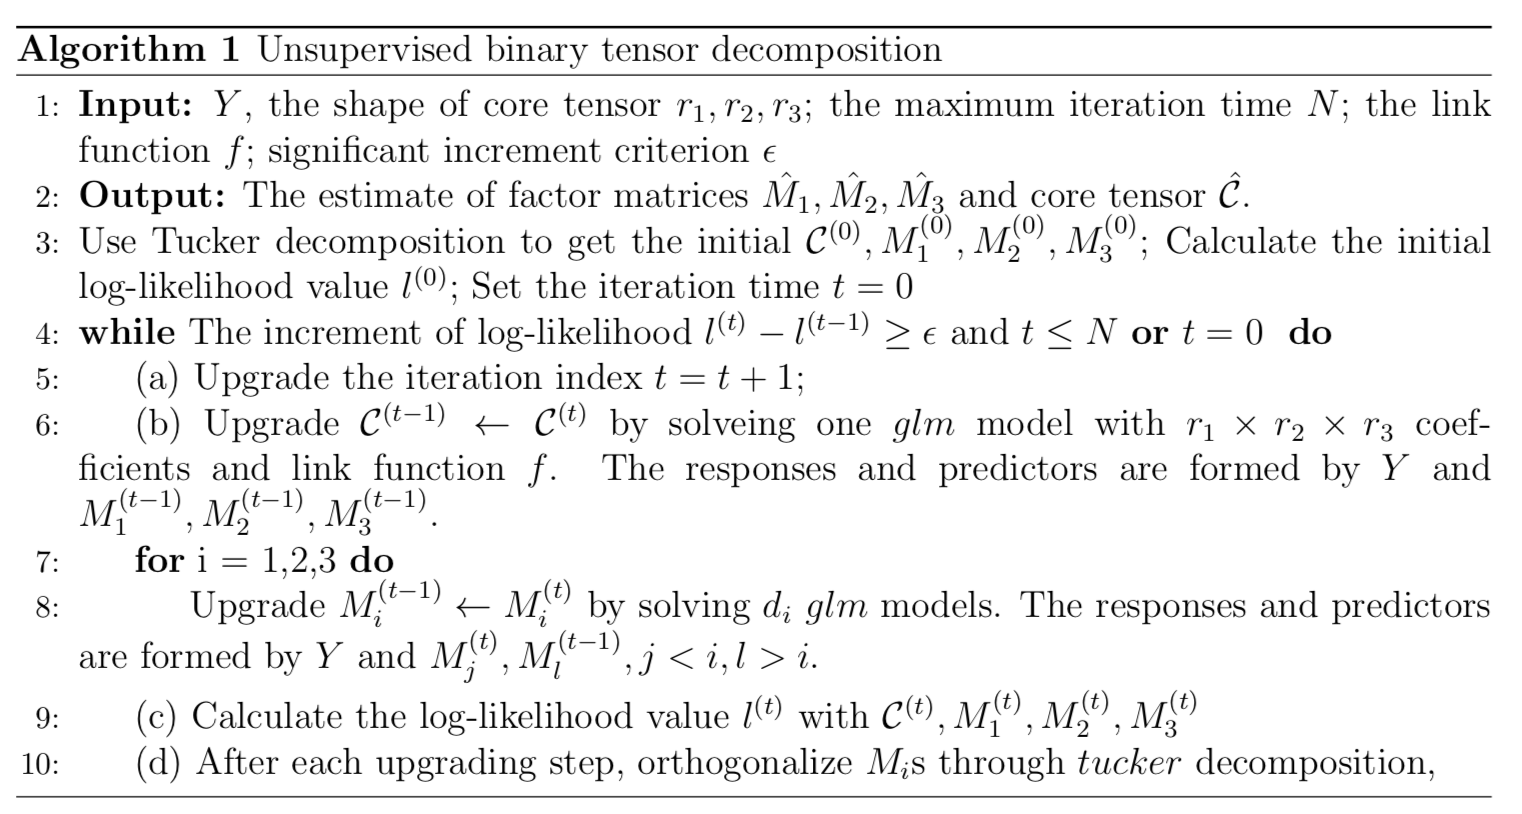
\includegraphics[width=17.5cm]{unsupervised.png}
  \end{center}
  \end{figure*}
  
We focus on the high-dimensional region in which both $d_k\to \infty$ and $p_k\to\infty$ while ${p_k\over d_k} \to \gamma_k \in[0,1]$. 
\begin{assumption}\label{ass}We make the following assumptions:
\vspace{-.5cm}
\begin{enumerate}
\item [1.] There exists two positive constants $c_1,\ c_2>0$ such that $c_1\leq \sigma_{\min}(\mX_k)\leq  \sigma_{\max}(\mX_k)\leq c_2$ for all $k\in[K]$.
\item [2.] There exist two positive constants $L,\ U>0$ such that $L\leq \text{Var}(y_{i_1,\ldots,i_K}|\tX)\leq U$ uniformly over the parameter space $\tP$. 
\item [2'.] Equivalently, $L\leq b''(x) \leq U$ for all $x\leq \alpha$, where $b(\cdot)$ is the known function in the exponential family distribution and $\alpha$ is the upper bound of the linear predictor. 
\end{enumerate}
\end{assumption}

  
\begin{thm}[Convergence]\label{thm:main}
Consider a generalized tensor regression model with multi-sided covariates. Let $\tY\in\mathbb{R}^{d_1\times \cdots\times d_K}$ be the tensor response and $\tX=\{\mX_1,\ldots,\mX_K\}$ the covariates, where $\mX_k\in\mathbb{R}^{p_k\times d_k}$ is the covariate matrix on mode-$k$. Suppose the entries in $\tY$ are independent realizations of an exponential family distribution, and $\mathbb{E}(\tY|\tX)$ follows the low-rank tensor regression model~\eqref{eq:tensormodel}. Under Assumption~\ref{ass}, there exist two constants $C_1, C_2>0$ such that, with probability at least $1-\exp(-C_1\sum_k p_k)$, 
\[
\text{Loss}(\trueB, \hat \tB) \leq  {C_2\sum_k p_k \over \prod_k d_k},
\]
where $C_2=C_2(\alpha, K, r_1,\ldots,r_K)>0$ is a constant that does not depend on dimension $\{d_k\}$ and $\{p_k\}$. 
\end{thm}

To gain further insight on the bound~\label{thm:main} we consider the special case when $d_1=d_2=\ldots=d_K=d$ . 1. binary case; 2. large dimension region. $\tO\left({p \over d^k}\right)\leq \tO(d^{-(k-1)})$.

\begin{cor}[Spatio-temporal growth model] Our method yields the convergence rate $\tO\left({p+r+s\over dmn}\right)$. Note that $p\leq d$, $r\leq m$ and $s\leq m$, so consistent estimator. 
\end{cor}

\begin{cor} [Network population model] Our method yields the convergence rate $\tO\left({2d+p\over d^2n}\right)$. Note that $p\leq m$, so this is a consistent estimator. In contrast, a naive repeated glm will give $\tO({p\over n})$.
\end{cor}

\begin{cor} [Link model with node attributes] Our method yields the convergence rate is $\tO\left({p\over d^2}\right)$. Note that $p\leq m$, so again a consistent estimator. In contrast, a naive repeated glm will give $\tO({p\over n})$.
\end{cor}

We provide the prediction accuracy for the response tensor.  
\begin{thm} [Prediction error]
Assume the same set-up as in Theorem~\eqref{thm:main}. Let $\mathbb{P}_{\tY_{\text{true}}}$ the distribution of $\tY$ given the true $\trueB$ and $\mathbb{E}(\tY|\tX)$ the true mean. Let $\mathbb{P}_{\hat \tY}$ denote the distribution given the estimated $\hat \tB$ and $\widehat{\mathbb{E}(\tY|\tX)}$ the predicted mean. We have, with probability at least $1-\exp(C_1\sum_k d_k)$,
\begin{align}
&\text{KL}(\mathbb{P}_{\tY_{\text{true}}},\ \mathbb{P}_{\hat \tY})\leq  C(...) {\sum_k p_k\over \prod_k d_k},\\
&\text{Loss}\left(\mathbb{E}(\tY|\tX),\ \widehat{\mathbb{E}(\tY|\tX)}\right)\leq b''(\alpha)C(...) {\sum_k p_k\over \prod_k d_k}.
\end{aligh}
\end{thm}

\subsubsection{Comparison between Gaussian and non-Gaussian models}

\section{Numerical implementation}
\subsection{Alternating optimization}
\subsection{Tuning parameter selection}\label{sec:tuning}
We propose to use Bayesian information criterion (BIC) and choose the rank that minimizes BIC; i.e.
\begin{align}
\hat \mr&=\argmin_{\mr=(r_1,\ldots,r_K)} \text{BIC}(\mr)\\
&=\argmin_{\mr=(r_1,\ldots,r_K)}\left[-2\tL_{\tY}(\hat \tB)+p_e(\mr)\log \left(\prod_k d_k\right) \right],
\end{align}
where $p_e(\mr)\stackrel{\text{def}}{=}\sum_k (d_k-1)r_k+\prod_k r_k$ is the effective number of parameters in the model. We choose $\hat \mr$ that minimizes $\text{BIC}(\mr)$ via grid search. Our choice of BIC aims to balance between the goodness-of-fit for the data and the degree of freedom in the population model. We test its empirical performance in Section~\ref{sec:simulation}.  

\section{Simulation}\label{sec:simulation}
\section{Data analysis}
\section{SUPPLEMENTARY MATERIAL}

If you need to include additional appendices during submission, you
can include them in the supplementary material file.



\section{INSTRUCTIONS FOR CAMERA-READY PAPERS}

For the camera-ready paper, if you are using \LaTeX, please make sure
that you follow these instructions.  (If you are not using \LaTeX,
please make sure to achieve the same effect using your chosen
typesetting package.)

\begin{enumerate}
    \item Download \texttt{fancyhdr.sty} -- the
    \texttt{aistats2020.sty} file will make use of it.
    \item Begin your document with
    \begin{flushleft}
    \texttt{\textbackslash documentclass[twoside]\{article\}}\\
    \texttt{\textbackslash usepackage[accepted]\{aistats2020\}}
    \end{flushleft}
    The \texttt{twoside} option for the class article allows the
    package \texttt{fancyhdr.sty} to include headings for even and odd
    numbered pages. The option \texttt{accepted} for the package
    \texttt{aistats2020.sty} will write a copyright notice at the end of
    the first column of the first page. This option will also print
    headings for the paper.  For the \emph{even} pages, the title of
    the paper will be used as heading and for \emph{odd} pages the
    author names will be used as heading.  If the title of the paper
    is too long or the number of authors is too large, the style will
    print a warning message as heading. If this happens additional
    commands can be used to place as headings shorter versions of the
    title and the author names. This is explained in the next point.
    \item  If you get warning messages as described above, then
    immediately after $\texttt{\textbackslash
    begin\{document\}}$, write
    \begin{flushleft}
    \texttt{\textbackslash runningtitle\{Provide here an alternative
    shorter version of the title of your paper\}}\\
    \texttt{\textbackslash runningauthor\{Provide here the surnames of
    the authors of your paper, all separated by commas\}}
    \end{flushleft}
    Note that the text that appears as argument in \texttt{\textbackslash
      runningtitle} will be printed as a heading in the \emph{even}
    pages. The text that appears as argument in \texttt{\textbackslash
      runningauthor} will be printed as a heading in the \emph{odd}
    pages.  If even the author surnames do not fit, it is acceptable
    to give a subset of author names followed by ``et al.''

    \item Use the file sample\_paper.tex as an example.

    \item The camera-ready versions of the accepted papers are 8
      pages, plus any additional pages needed for references.

    \item If you need to include additional appendices,
      you can include them in the supplementary
      material file.

    \item Please, don't change the layout given by the above
      instructions and by the style file.

\end{enumerate}

\subsubsection*{Acknowledgements}

Use the unnumbered third level heading for the acknowledgements.  All
acknowledgements go at the end of the paper.

\subsubsection*{References}

References follow the acknowledgements.  Use an unnumbered third level
heading for the references section.  Any choice of citation style is
acceptable as long as you are consistent.  Please use the same font
size for references as for the body of the paper---remember that
references do not count against your page length total.

\begin{thebibliography}{}
\setlength{\itemindent}{-\leftmargin}
\makeatletter\renewcommand{\@biblabel}[1]{}\makeatother
\bibitem{} J.~Alspector, B.~Gupta, and R.~B.~Allen (1989).
    \newblock Performance of a stochastic learning microchip.
    \newblock In D. S. Touretzky (ed.),
    \textit{Advances in Neural Information Processing Systems 1}, 748--760.
    San Mateo, Calif.: Morgan Kaufmann.

\bibitem{} F.~Rosenblatt (1962).
    \newblock \textit{Principles of Neurodynamics.}
    \newblock Washington, D.C.: Spartan Books.

\bibitem{} G.~Tesauro (1989).
    \newblock Neurogammon wins computer Olympiad.
    \newblock \textit{Neural Computation} \textbf{1}(3):321--323.
\end{thebibliography}
\end{document}
